\section{Data Analysis}
\label{sec:Analysis}
In this work we re-analyze science run~II data recorded between February 2011 and March 2012, 
corresponding to 224.6~live~days. The characterization of the detector response to ER interactions is performed using dedicated calibration campaigns with $^{60}$Co and $^{232}$Th radioactive sources, while the response to NR interactions is performed using $^{241}$AmBe neutron source calibration campaigns.
 
This work extends the previous results~\cite{xe100_run10_si,xe100_run_combination}, referred to in the following as the low-energy channel, with a new study exploring the recoil energy range between $43-240~\keVr$. 
The data analysis is divided into two mutually exclusive channels, one optimized for low energies and ranging from 3-30~PE in \cSi{} (low-energy), 
the other optimized for high energies recoils ranging from 30-180~PE in \cSi{} (high-energy). These two analyses are then combined statistically. 

\subsection{Low Energy Channel}
\label{subsec:LowE}
This analysis channel relies on the re-analysis of run~II data described in~\cite{xe100_run_combination}. The region of interest (ROI), the background 
expectation models, data selections and their acceptances are mostly unchanged and so are only briefly summarized here. Differences with respect to said results are highlighted when present.

The ROI for this channel is defined in the ($y,cS1$)-plane and is shown in Figure~\ref{fig:phasespace}.  The lower 
bound on $y$ corresponds to a 3\,$\sigma$ acceptance quantile (as a function of cS1) of a 20~GeV WIMP mass signal model assuming an $\mathcal{O}_1$ (SI) interaction, while the upper bound is fixed at y\,=\,2.7.
The range in cS1 is selected as 3 to 30\,PE. 
The ROI is further divided into eight sub-regions (also called bands) depending on the operator $\mathcal{O}_i$ and on the WIMP mass hypothesis. 
These bands are arranged to achieve constant expected signal density in each region, as described in~\cite{xe100_run_combination}.

\begin{figure}[]
\begin{minipage}{1\linewidth}
\centerline{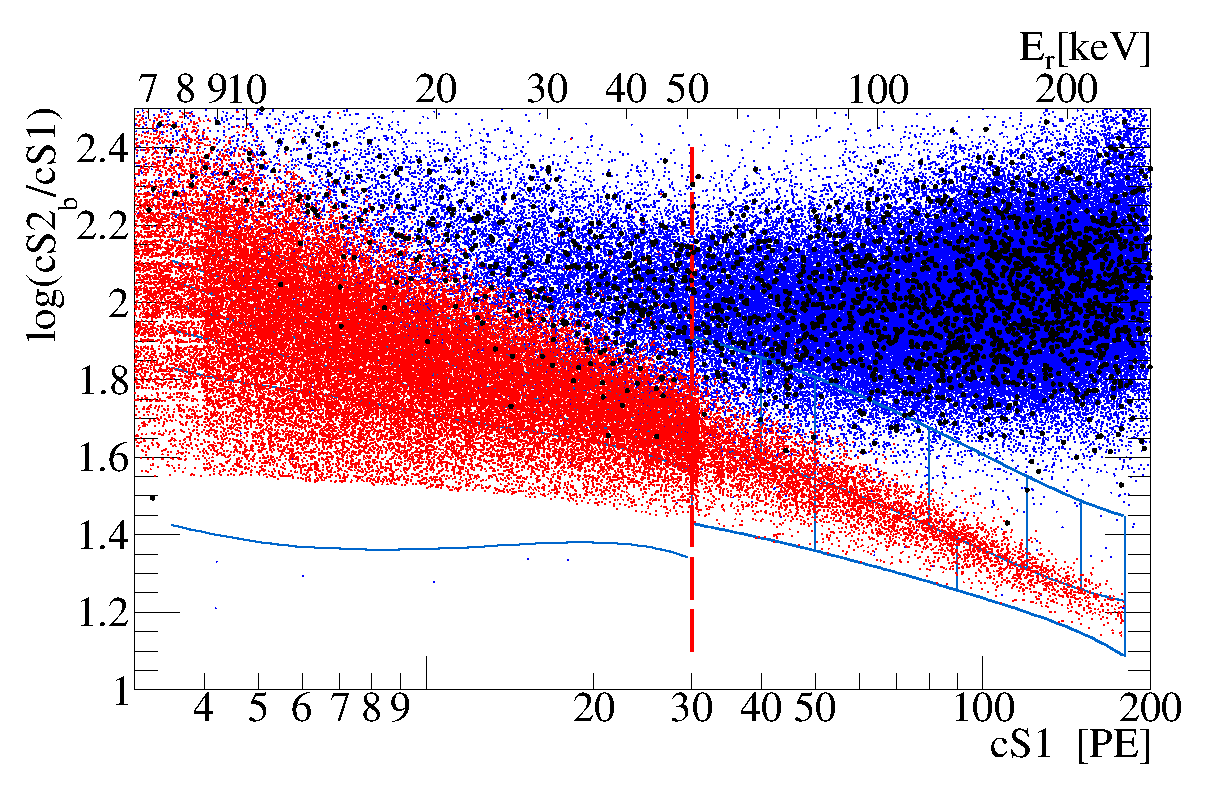
\includegraphics[width=1\linewidth]{Figures/eft_sr.eps}}
\end{minipage}
\caption{Summary of regions of interest, backgrounds, and observed data. ER calibration data, namely $^{60}\mathrm{Co}$ and $^{232}\mathrm{Th}$ data is shown as blue dots. NR calibration data ($^{241}$AmBe) is shown as red dots. Dark matter search data is shown as black dots. The red dashed line is the threshold between the low and high energy channels. The lines in blue are the bands. For the low-energy channel these are operator and mass dependent, but are shown here for a 50~GeV/$c^2$ WIMP using the $\mathcal{O}_1$ operator. For the high-energy region, the nine analysis bins are presented also in blue lines.
%\sout{the top left bin in this region is bin 1, the top right is bin 6, the bottom left is bin 7 and bottom right is bin 9. 
%In Sec.~\ref{sec:Results} we show similar data but for regions above the upper range of this analysis, going up to 1000\,PE in cS1, for completeness as part of final unblinding of XENON100 data.} 
}
\label{fig:phasespace}
\end{figure}  


Other than falling into the ROI, an event should fulfill several additional selection criteria (cuts). Data quality and selection cuts are defined to remove events with poor data quality or noisy signals. \ale{Events are discarded if they present} a time-coincident signal in the outer LXe veto, S2 signals below threshold, multiple-scatters, or are localized outside a predefined fiducial volume of 34 kg. In addition, this analysis channel uses the post-unblinding cuts and data reprocessing described in~\cite{xe100_run_combination}. More details on these selection criteria and their relative WIMP signals acceptances can be found in~\cite{Aprile:2012vw,xe100_run_combination}. 
%%%%% MAYBE THIS CAN BE COMMENTED OUT %%%%%%
%%% Ale : already sayd above, and is not "new features" of this analysis.
%\sout{To summarize the main new features in this analysis, data is reprocessed with an improved (S1,S2) classification algorithm, and a new cut targeted to suppress data periods with non-random occurrence of lone-S1 (an S1 without 
%any correlated S2) events is applied.} 
%%%%%%%%%%%%%%%%%%%%%%%%%%%%%%%%%%%%%%%%%%%%%
\ale{Note that}
%Finally, 
this analysis channel does not employ a variable lower S1 threshold as a function of the event position in the TPC, but instead applies a fixed lower threshold cut on cS1 at 3\,PE, \ale{conversely} to the choice made in~\cite{xe100_run_combination}.

The expected background is modeled separately for ER and NR contributions which are then scaled to exposure and added together.
The NR background is estimated by Monte Carlo simulation and accounts for the radiogenic and cosmogenic neutron
contributions~\cite{Aprile:2013tov}. The ER background is parametrized as the linear combination of Gaussian-shaped and non-Gaussian components.
The first is obtained via a parametric fit of the $^{60}$Co and $^{232}$Th calibration data, as discussed in~\cite{xe100_run10_si}.
%In contrast, the expected distribution and yields for the non-Gaussian population, 
\ale{The second, } consisting of anomalous events such as those 
presenting incomplete charge collection or accidental coincidence of uncorrelated S1s and S2s,  
is evaluated via dedicated techniques described in~\cite{xe100_run_combination}.

\ale{Systematic uncertainties on the background model arising from the Gaussian parametrized fit, from the normalizations of the NR and from the non-Gaussian components, have been evaluated and propagated to each band}. \BenComment{*This sentence doesn't make sense; missing an "and" or something? I can't quite guess what it is supposed to mean*} These errors are small with respect to the statistical uncertainties of each band, which are conservatively taken as the overall uncertainty~\cite{xe100_run_combination}, as discussed in Sec.~\ref{sec:LikelihoodFunction}.



\subsection{High energy channel}
\label{subsubsec:HighE}
This analysis channel targets high energy nuclear recoils and is the focus of this work. The data selection criteria used are based on the criteria described in detail in \cite{Aprile:2012vw}, which were optimized for high acceptance to low energy nuclear recoils. Most of these cuts were found to be fully compatible with (or easily extended) to high energy depositions, however some required more comprehensive studies, which are described in the following . 

The width of an \Sii{} pulse increases with the depth (z) of the interaction. This is due to the diffusion of the electron cloud during its propagation
through the liquid xenon. Since low energy \Sii{} events show larger spread
due to low statistics of drifted electrons, the cut was previously defined in an energy-dependent way. However, for the large recoil energies considered in this channel, this energy dependency is no longer valid. We therefore use here a cut on the \Sii{} width which is a function of the depth of the interaction alone. 

As a WIMP will interact only once in the detector, we remove events which have more than one \Sii{}. We adopt in this analysis a cut that is more suitable to higher energies and demand a single \Sii{} in a 160 $\mu$s window, instead of a linear dependence between the second \Sii{} size and the first. 

To define the interaction's exact location in ($x,y$), we use several algorithms, one of which is based on a Neural Network (NN)~\cite{Aprile:2012vw}. The NN was not trained to recognize high energy ER events and therefore a cut on the NN reconstruction quality is not suitable for this analysis. We therefore discard this cut but keep all other selections on position reconstruction quality, which is sufficient to ensure a correct position reconstruction. 

The total acceptance to WIMP signals is computed based on $^{241}$AmBe calibration data as a function of \cSi, following the procedure described in~\cite{Aprile:2012vw}. We present this function in Figure~\ref{fig:Acc}, where the total acceptance is fitted using a third order polynomial.

\begin{figure}[t!]
\begin{minipage}{0.9\linewidth}
\centerline{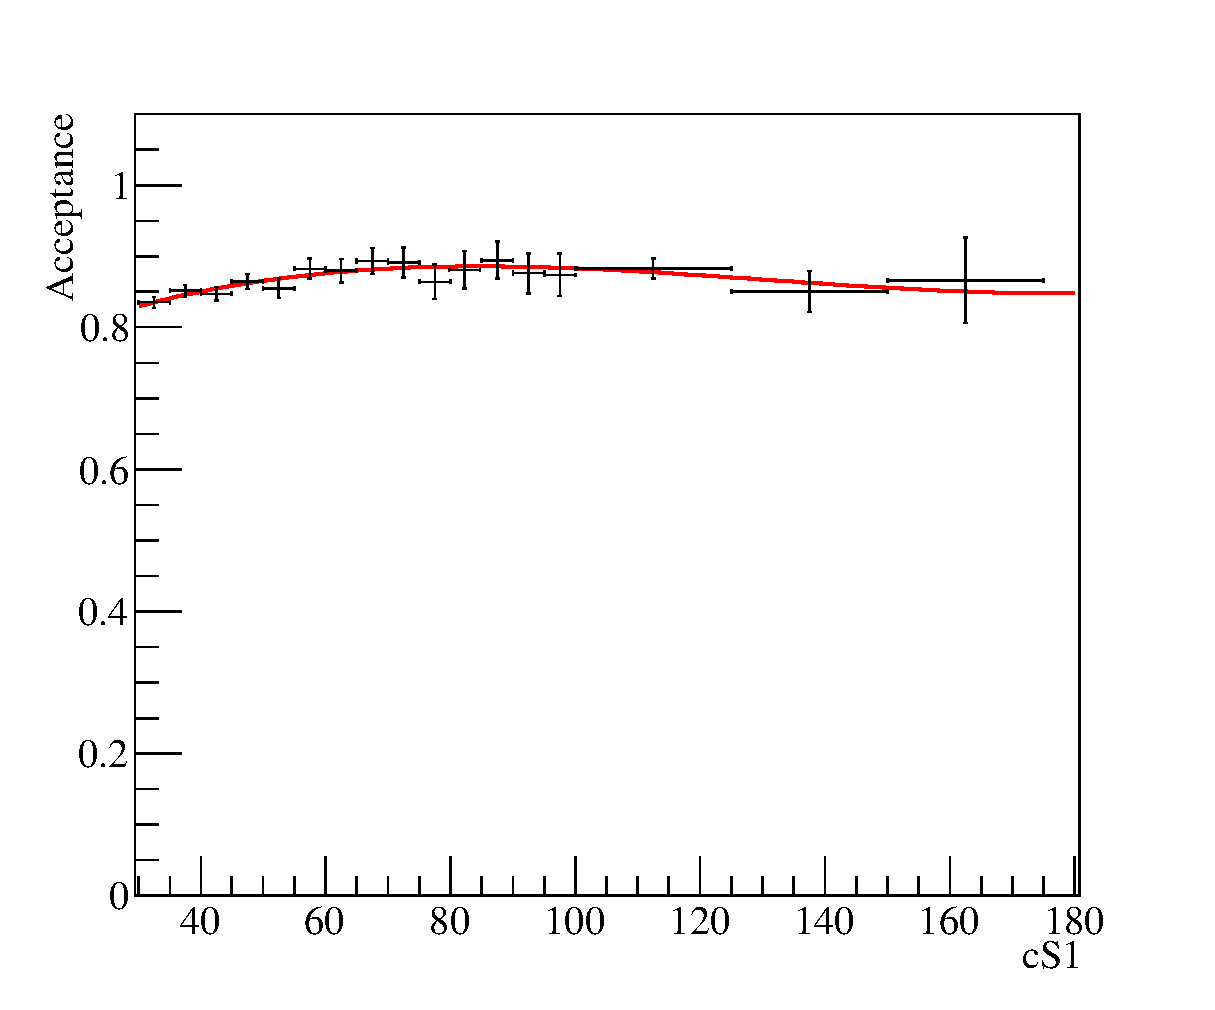
\includegraphics[width=1.\linewidth]{Figures/Acceptance.eps}}
\end{minipage}
\caption{The total acceptance of all cuts used. Data from calibration is shown in black, with a 3rd order polynomial fit in red.}
\label{fig:Acc}
\end{figure}

We define our signal region in the discrimination $(y,\cSi)$-plane using $^{241}$AmBe calibration data. 
The region of interest is shown in Figure~\ref{fig:phasespace} as blue contour lines. The upper bound in $y$ is defined such that the contribution due to xenon inelastic interaction lines is negligible. The lower bound is defined as the 3\,$\sigma$ acceptance quantile of the $^{241}$AmBe distribution.

We divide our signal region into two bands in $y$, constructed such that the $^{241}$AmBe data sample is equally distributed in between them. The number of events in each band is $\sim3000$. The bands are further divided into nine bins, the number and boundaries of which have been optimized via Monte-Carlo (MC) simulation. The definitions of the bins boundaries are presented in Table~\ref{table:BinDef} and in Figure~\ref{fig:phasespace}. 

The main source of background results from ER leakage. We therefore estimate the background distribution in the ROI using $^{60}$Co and $^{232}$Th calibration events.  
Contributions from radiogenic and cosmogenic neutrons, as well as accidental coincidence, are negligible for such a high energy recoil. In Table~\ref{table:BinDef} we report the 
background expectation in the ROI along with the observed events for each bin.
Here the background expectation is computed by scaling the calibration sample yield by $6.54\times10^{-3}$, which is the ratio of observed counts to calibration counts in an independent sideband. The sideband is defined above the upper limit of this analysis and below the ER calibration band mean. Note that in the computation of exclusion limits, the background normalization is fitted to data, rather than using the sideband normalization, as described in section~\ref{sec:LikelihoodFunction}. 

%%%%%%%%%%%%%%%%%%%%%%%%%%%%%%%%%%%%%%%%%%%%%%%%%%%%%%%%%%%%%%%%%%%%%%%%%%%%%%%%%%%%%%%%%%%%%%%%%%%%%%%


\begin{table}
\resizebox{1.\columnwidth}{!}{

	 \begin{tabular}{ c c c c c c } 
 \hline\hline
 \# & Band  & Energy Range $(\cSi)$  & \# Background Events & \# Data Events \\  
 \hline
 1 & upper & 30  - 40  & 23.5$\pm$5.1 & 20 \\ 
 
 2 & upper & 40  - 50  & 15.7$\pm$3.5 & 17 \\
 
 3 & upper & 50  - 80  & 12.4$\pm$2.8 & 11 \\
 
 4 & upper & 80  - 120 & $1.1\pm0.3$  & 1  \\
 
 5 & upper & 120 - 150 & $(1.0\pm0.5)\times 10^{-1}$  & 1  \\  
 
 6 & upper & 150 - 180 & $(0.8\pm0.4)\times 10^{-1}$ & 0  \\  
 
 7 & lower & 30  - 50  & $0.9\pm0.3$  & 0  \\  
 
 8 & lower & 50  - 90 & $(3.5\pm1.2)\times 10^{-1}$ & 0  \\  
 
 9 & lower & 120 - 180 & $(1.8\pm0.7)\times 10^{-1}$& 0  \\  
 \hline\hline
\end{tabular}
}

\caption{Definitions and contents of the analysis bins for the high energy channel. The expected background counts are calculated by taking the calibration sample and scaling it by $6.54\times10^{-3}$, which is the ratio of observed counts to calibration counts in a sideband.}  \label{table:BinDef} 
\end{table}






\subsection{Signal model}
\label{subsec:SignalModel}
The signal model is produced by taking a theoretical event rate spectrum, the production of which is described in sections \ref{subsubsec:Elastic} and \ref{subsubsec:Inelastic}, and applying the analysis acceptance and detector response as described in ~\cite{Aprile:2012vw}  to obtain the expected event rate in the detector in terms of detector variables (i.e. \cSi{}, \cSiib{}). 
In both analysis channels, we use Eq.~\ref{eq:LeffEnergyScale} in order to compute the expected average \cSi{} for a given NR energy,
\begin{equation}
\label{eq:LeffEnergyScale}
	\langle \cSi \rangle = E_{\mathrm{nr}} \cdot (\Ly \Leff) \cdot   \left(\frac{S_\mathrm{nr}}{S_\mathrm{ee}}\right) 
\end{equation}

where $E_\mathrm{nr}$ is the recoil energy, $\Ly$ is the average light yield in the detector, $\Leff$ is the scintillation efficiency relative to 122$\keVee$ as a function of $E_\mathrm{nr}$, and $S_\mathrm{ee}$ and $S_\mathrm{nr}$ are the quenching factors due to the externally applied electric field. Aside from $E_\mathrm{nr}$ and $\Leff$ these parameters have fixed values, namely $\Ly = 2.28 \pm 0.04$, $S_\mathrm{nr} = 0.95$, and $S_\mathrm{ee} = 0.58$. Recoils below $3~\keVr$ are assumed to produce no light. For details of the physics behind these parameters and the construction of the signal probability density function (PDF) please see \cite{Aprile:2012vw,xe100_run_combination}. 

For the low-energy region, the expected \cSiib{} signal is computed following~\cite{DataMCXenon} using Eq.~\ref{eq:Qy},


\begin{equation}
\label{eq:Qy}
	\langle \cSiib \rangle = E_{\mathrm{nr}}\Qy Y   
\end{equation}
where $Y = 8.3 \pm 0.3$ 
is the amplification factor determined from the detector response to single electrons~\cite{XenonSingleElectron}, and $\Qy$ is the charge yield as a function of $E_\mathrm{nr}$. Applying the detector and PMT responses, and the acceptance as in \cite{xe100_run_combination}, defines the low-energy signal model over the region $3~\mathrm{PE} < \cSi{} < 30~\mathrm{PE}$, with $\cSiib{} > 73.5~\mathrm{PE}$ as the \Sii{} threshold.

Eq. \ref{eq:Qy} hides a subtlety. The actual \cSiib{} PDF is composed of two pieces, a Poisson term associated with the initial charge liberation and a Gaussian term associated with the PMT response and other detector effects:
%
\begin{equation}
\label{eq.cS2pdf}
p_\mathrm{S2}(\mathrm{\cSiib}|E) = \sum_{N'} P_\mathrm{pmt}(\mathrm{\cSiib}|Y N',\sigma_Y \sqrt{N'})\cdot\mathrm{Pois}(N'|\mu_Q)
\end{equation}
%
where $\mu_Q=E_{\mathrm{nr}}\Qy$ is the expected number of liberated charges in a nuclear recoil event of energy $E$, and $N'$ is the actual number of liberated charges. The amplification factor $Y$ is applied to the actual number of liberated charges $N'$, not the expected number $\mu_Q$. Associated with this is the variance of the Gaussian response PDF, $\sigma_Y\sqrt{N'}$, where in this analysis $\sigma_Y = 6.93$ as measured and described in~\cite{XenonSingleElectron}. 
%%%%%%%%%%%%%%%%%%%%%%%%%%%%%%%%%%%%%%%%%%%%%%%%%%%%%%%%%%%%%%%%%%%%%%%%%%%%%%%%%%%%%%%%%%%%%%%%%%%%%%%%%%%%%%%%%%

For the high energy region we cannot produce the \Sii{} distribution in the same way as the method in~\cite{DataMCXenon}, since it  has not been calibrated for such high recoil energies. We therefore use the NR calibration data distribution in log($\mathrm{\cSiib/\cSi}$) to estimate the WIMP distribution. Above 180~PE in \cSi{}, the event yield of $^{241}$AmBe data is too low to estimate the distribution accurately. This forms the upper bound of this analysis. With the \cSiib{} distribution determined by this empirical method, we require only a prediction of the \cSi{} distribution. This is obtained from Equation (\ref{eq:LeffEnergyScale}), followed by the application of detector and PMT responses, as well as the acceptance given in Figure~\ref{fig:Acc}, which completes the high-energy signal model definition.

Figures ~\ref{fig:HighE} and \ref{fig:LowE} shows dashed signal distribution examples for two EFT operators and for the low and the high energy region, respectively.
In both cases, the signal distributions are normalized to yield 5 events in the total energy range (low-energy and high-energy).

\begin{figure}[h!]
\begin{minipage}{1.\linewidth}
\centerline{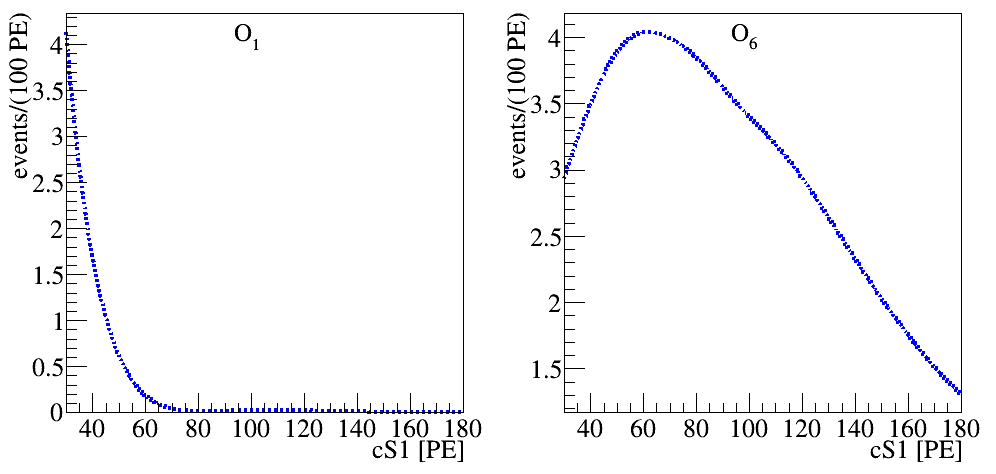
\includegraphics[width=1.\linewidth]{Figures/SigHighO1O6.png}}
\end{minipage}
\caption{The expected signal in the high energy region for a 300~GeV/$c^2$ WIMP mass, normalized to 5 events. Left(right) is the spectra for $O_1$($O_6$). Notice that for $O_1$ most of the events are not expected to deposit energy higher than 30~PE whereas for $O_6$ a large fraction of the events appear in this region.}
\label{fig:HighE}
\end{figure} 

\begin{figure}[h!]
\begin{minipage}{1.\linewidth}
\centerline{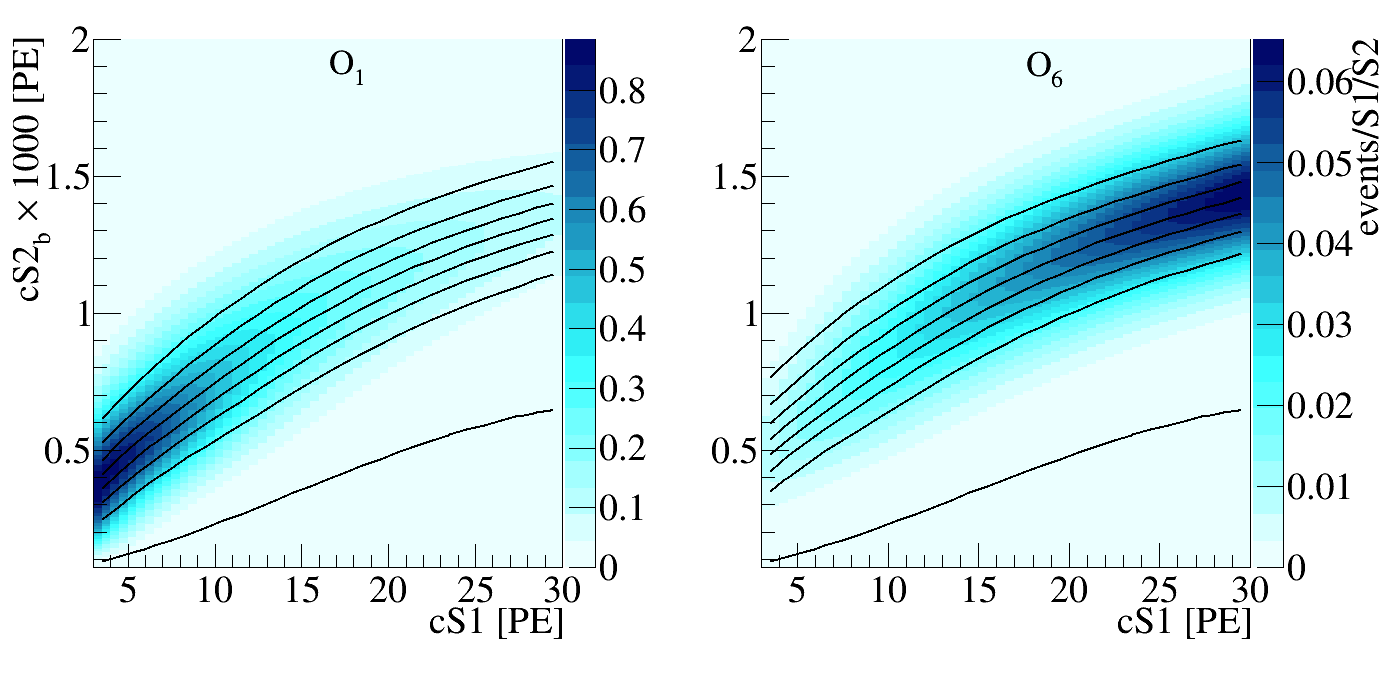
\includegraphics[width=1.\linewidth]{Figures/SigLowO1O6.png}}
\end{minipage}
\caption{The expected signal in the low energy region for a 300~GeV/$c^2$ WIMP mass, normalized to 5 events. Left(right) is the spectra for $\mathcal{O}_1$($\mathcal{O}_6$). Notice that for $\mathcal{O}_1$ most of the events are expected to deposit energy lower than 30~PE whereas for $\mathcal{O}_6$ a large fraction of the events do not appear in this region at all. The black lines indicate the bands constructed on these specific mass and operator models, and are dividing the signal into 8 equally distributed signal sub-regions. This parameter space can be mapped with a one to one mapping to the $(y-\cSi)$ space.}
\label{fig:LowE}
\end{figure}




\subsubsection{Elastic scattering}
\label{subsubsec:Elastic}

The expected recoil energy spectrum of each WIMP mass for each EFT operator is calculated using the Mathematica package \texttt{DMFormFactor} supplied by Anand et. al.~\cite{Fitzpatrick:MathTools,Anand:MathTools}. We use standard assumptions as in previous analyses (e.g \cite{xe100_run_combination}) regarding the local dark matter density and velocity distribution, namely $\rho_\mathrm{local} = 0.3$~GeV$\cdot c^{-2}$/$\mathrm{cm}^{3}$ and a Maxwell-Boltzman distribution with a mean given by the local circular velocity $v_0 = 220$ km/s and cut off at an escape velocity of $v_\mathrm{esc} = 544$ km/s. The responses of xenon nuclei to a scattering event are computed from one-body density matrices provided with the package, in contrast to the Helm form factors which have been used in previous analyses. These spectra are produced for the seven most abundant xenon isotopes (128, 129, 130, 131, 132, 134 and 136), combined in proportion to the abundance of these isotopes in the XENON detector \cite{xe100_run10_sd}, then translated into expected signal rates via the method described above.

\subsubsection{Inelastic WIMP scattering}
\label{subsubsec:Inelastic}
To obtain recoil spectra for WIMP-nucleon scattering for all EFT operators with inelastic kinematics, we use a modified version of \texttt{DMFormFactor} provided by Barello et. al. \cite{InelasticMath}. The authors have modified the original package to enforce the new energy conservation condition $\delta_m + \vec{v}\cdot\vec{q} + \left|\vec{q}\right|^2/2\mu_N = 0$, primarily by replacing 
$\vec{v}^\perp_{elastic} \rightarrow \vec{v}^\perp_{inelastic} = \vec{v}^\perp_{elastic} +\frac{\delta_m}{\vert{\vec{q}}\vert^2}\vec{q}$ in the definitions of the EFT and nuclear operators, giving rise to the well-known minimum velocity for scattering
\begin{equation}
  v_\mathrm{min}/c = \frac{1}{\sqrt{2 m_N E_R}} \left|\frac{m_N E_R}{\mu_N} + \delta_m\right|
\end{equation}
where $\mu_N$ is the WIMP-nucleon reduced mass.

Assumptions regarding the dark matter halo and nuclear physics are unchanged. The mass splitting $\delta_m$ between dark matter states is varied from 0 to 300 keV, safely beyond the value at which the predicted rate is zero for the entire mass range we consider.
